\chapter{Αλγόριθμος \textlatin{Bayes} } \label{experimentationANDresults}

\section{Θεμελιώδης στατιστική \textlatin{Bayes}} 
%-Bayesian foundation and implementation [Loredo 2004, Feroz & Hobson 2008]
Προκειμένου να καταλήξουμε σε ένα συμπέρασμα υπολογίζουμε πιθανότητες της υπόθεσης που μας ενδιαφέρει- η οποία ποσοτικοποιείται σε ένα σετ παραμέτρων $\Theta$- έχοντας διαθέσιμα δεδομένα $D$ και έχοντας υποκείμενες εικασίες- δηλαδή ένα μοντέλο $Μ$. Το θεώρημα \textlatin{Bayes} εκφράζει την εκ των υστέρων αυτή πιθανότητα (\textlatin{posterior probability})\cite{Loredo}: 
\begin{equation}\begin{aligned} p (\Theta |D,M)= \dfrac{ p (\Theta |M) \cdot p (D |\Theta ,M) }{ p (D|M)}  \label{eq:BayesTheorem}\end{aligned}\end{equation}
Όπου:\\
-$p (\Theta |D,M)$ : η εκ των υστέρων κατανομή πιθανότητας για τις παραμέτρους $\Theta$ (\textlatin{posterior probability}- στο εξής θα αναφερόμαστε σε αυτήν ως \textlatin{posterior}).\\
-$p (\Theta |M)$ : η εκ των προτέρων κατανομή πιθανότητας για τις παραμέτρους $\Theta$ (\textlatin{prior probability}- στο εξής θα αναφερόμαστε σε αυτήν ως \textlatin{prior}).\\
-$p (D |\Theta ,M)$ : η δειγματοληπτική κατανομή των δεδομένων $D$ δηλαδή το ενδεχόμενο να παρατηρήσουμε τα δεδομένα $D$ θεωρώντας μοντέλο $Μ$ με παραμέτρους $\Theta$ (\textlatin{likelihood}- στο εξής θα αναφερόμαστε σε αυτήν ως \textlatin{likelihood}).\\
-$p (D|M)$ : η <<προγνωστική>> κατανομή δεδομένων, $Ζ$ (\textlatin{evidence}- στο εξής θα αναφερόμαστε σε αυτήν ως \textlatin{evidence}).

Στην συμπερασματολογία (εκτίμηση παραμέτρων) ενδιαφερόμαστε για το πώς η \textlatin{posterior} $p (\Theta |D,M)$ μεταβάλεται με τις παραμέτρους $\Theta$ όταν τα δεδομένα $D$ έχουν σταθερές τιμές. Οπότε, μεγαλύτερη σημασία έχει το πώς η δειγματοληπτική κατανομή $p (D |\Theta ,M)$ μεταβάλεται με τις μαραμέτρους $\Theta$, και όχι μετα δεδομένα $D$, γι> αυτό την ονομάζουμε ενδεχόμενο για τις $\Theta$ (\textlatin{likelihood}) $\mathcal{L}\equiv p (D |\Theta ,M)$. Η \textlatin{evidence} $p (D|M)$ δεν έχει εξάρτηση από τις παραμέτρους $\Theta$ έτσι, λοιπόν, έχει τον ρόλο κανονικοποιητικού παράγοντα για την $\textlatin{posterior}$ που υπολογίζεται ως τέτοιος: \begin{equation}\begin{aligned} p (D|M) = \int_{\Omega_\Theta}  p (D |\Theta ,M)\cdot p (\Theta |M)   d\Theta \label{eq:evidence}\end{aligned}\end{equation}
Η \textlatin{posterior} $p (\Theta |D,M)$ συνιστά την πλήρη συμπερασματολογία \textlatin{Bayes} για τις τιμές των παραμέτρων και μπορεί να ολοκληρωθεί για κάθε παράμετρο. Αν χωρίσουμε τις $\Theta$ σε παραμέτρους που μας ενδιαφέρουν $\psi$ και αδιάφορες παραμέτρους $\phi$, τότε η συμπερασματολογία για τις $\psi$ είναι η ολοκληρωμένη κατανομή που προκύπτει ολοκληρώνοντας την \textlatin{posterior} ως προς τις παραμέτρους $\phi$\cite{Loredo}:
\begin{equation}\begin{aligned} p (\psi |D,M)=\int_{\Omega_\phi} p (\Theta |D,M) d\phi = \int_{\Omega_\phi} p (\psi , \phi |D,M) d\phi \label{eq:MarginalDistri}\end{aligned}\end{equation}
To θεώρημα \textlatin{Bayes} εφαρμόζεται τόσο για υπολογισμό \textlatin{posterior} κατανομών πυκνότητας πιθανότητας όσο και για διακριτές \textlatin{posterior} κατανομές πιθανότητας, όπου αντί για ολοκληρώματα έχουμε αθροίσματα.

\subsection{Τεχνικές δειγματοληψίας \textlatin{Markov Chain Monte Carlo (MCMC)}}

Ο αλγόριθμος δειγματοληψίας \textlatin{Markov Chain Monte Carlo (MCMC)} είναι μια μέθοδος \textlatin{Bayes} που χρησιμοποιείται για ολοκλήρωση και εκτίμηση παραμέτρων. Ο αλγόριθμος σε κάθε βήμα συγκρίνει ένα αρχικό σημείο με ένα τυχόν σημείο από μία αρχική κατανομή με τοπική μεροληψία. Με πιθανότητα ανάλογη του πηλίκου των δύο σημείων ο αλγόριθμος επιλέγει ένα νέο σημείο ως σημείο εκκίνησης του επόμενου βήματος. Με κάθε επανάληψη παράγεται ένα σημείο, οπότε δημιουργείται μία αλυσίδα που έχει την ιδιότητα να αναπαριστά τα ανύσματα παραμέτρων $\Theta$ σε αναλογία με την πιθανότητά τους. Αυτή η αναπαράσταση του παραμετρικού χώρου μπορεί να ολοκληρωθεί ως προς τις παραμέτρους που δεν μας ενδιαφέρουν για να εξετάσουμε την κατανομή των παραμέτρων που μας ενδιαφέρουν.  
Η διάδοση σφαλμάτων στις εξαγόμενες ποσότητες μπορεί να γίνει σχολαστικά χωρίς να υιοθετήσουμε σφάλματα κατανομής \textlatin{Gauss}\cite{BuchnerGeorgakakis}.
H συμπερασματολογία ακολουθώντας τεχνικές \textlatin{Markov Chain Monte Carlo (MCMC)} γίνεται με δείγματα από μη-κανονικοποιημένη \textlatin{posterior} με αποτέλεσμα στην ισορροπία να έχουμε μια αλυσίδα που περιέχει ένα δείγμα του παραμετρικού χώρου κατανεμειμένο σύμφωνα με την \textlatin{posterior} με μετρική που υπαγορεύει η \textlatin{prior} χωρίς όμως να είναι κανονικοποιημένη. 

\subsection{Αλγόριθμος ένθετης δειγματοληψίας \textlatin{Nested Sampling (NS)}}

Η συμπερασματολογία \textlatin{Bayes} ενέχει δύο υπολογιστικές προκλήσεις. Πρώτον, κατά την εκτίμηση των παραμέτρων $\Theta$ ενός μοντέλου $Μ$ για τα δεδομένα $D$ η \textlatin{posterior} κατανομή μπορεί να είναι πολυτροπική \textlatin{(multi-modal)}- τότε η σύγκλιση σε στατική κατάσταση (ισορροπία) της παραδοσιακής τεχνικής \textlatin{MCMC} γίνεται πολύ αργή. Δεύτερον, κατά την επιλογή μοντέλου, η κατανομή \textlatin{evidence} (σχέση \ref{eq:evidence}) ως κανονικοποιητικός παράγοντας πρέπει να υπολογιστεί- αυτό σημαίνει υπολογισμό πολυδιάστατων ολοκληρωμάτων στον παραμετρικό χώρο, όταν η μετρική του παραμετρικού χώρου δίνεται από την \textlatin{prior}.\\
Η τεχνική της ένθετης δειγματοληψίας \textlatin{(Nested Sampling, NS)} είναι μια σύγχρονη τεχνική \textlatin{Monte Carlo} που εστιάζει στον υπολογισμό του ολοκληρώματος αυτού και επιτρέπει τον υπολογισμο της \textlatin{posterior} κατορθώνοντας ταυτόχρονα και εκτίμηση παραμέτρων και επιλογή μοντέλου\cite{Feroz2019}.
Προτέρημα του αλγορίθμου \textlatin{nested sampling}, εκτός από τον υπολογισμό πολυδιάστατων ολοκληρωμάτων, είναι ο εύκολος χειρισμός συναρτήσεων δειγματοληπτικής κατανομής (\textlatin{likelihood}) που μπορεί να είναι πολυτροπικές ή με περίεργο σχήμα. Ο αλγόριθμος \textlatin{NS} εκτιμά ολοκληρώματα εντοπίζοντας πώς τμήμα του όγκου παραμετρικού χώρου (όγκο τον οποίο υπαγορεύει η \textlatin{prior}) συρρικνώνεται όταν σταδιακά αυξάνουμε το όριο της \textlatin{likelihood}. Η μείωση στην επιφάνεια (για \textlatin{prior} που ορίζει επιφάνεια παραμετρικού χώρου) σε ένα βήμα πολλαπλασιασμένη με το ύψος του βήματος στην \textlatin{likelihood} προσεγγίζει τον συνολικό όγκο αθροίζοντας, ανεξαρτήτως του σχήματος της επιφάνειας που αντιστοιχεί στο βήμα. Στην διαδικασία αυτή παράγει την \textlatin{posterior} πιθανότητα για τις παραμέτρους και υπολογίζει το ολοκλήρωμα στον παραμετρικό χώρο\cite{Buchner2014}. 
%Nested Sampling (NS, Skilling, 2004) is a Monte Carlo algorithm for com-puting the integral over a model parameter space. In the context of Bayesian inference, theintegrand is the likelihood function, which is marginalised over the parameter space accord-ing to the prior definition (which donates the space metric). The integralZis known as themarginal likelihood or Bayesian evidence. \cite{Buchner2021}

%%------------------------------------------%%

\section{Εφαρμογή συμπερασματολογίας \textlatin{Bayes} στον αλγόριθμο υπολογισμού της \textlatin{NXSV}}

%{\color{red} στον αλγοριθμο υπολογισμου της excess variance?}

Σε κάθε πηγή \textlatin{AGN} που μελετάμε αντιστοιχεί μια καμπύλη φωτός, κάθε σημείο της καμπύλης φωτός είναι μία παρατήρηση με καταγεγραμμένη διάρκεια και καταγεγραμμένο αριθμό φωτονίων σε δεδομένη ενέργεια και ανιχνευτικό μέσο.

Τα δεδομένα μας ($D$) είναι οι καταμετρήσεις φωτονίων για κάθε παρατήρηση (καταμετρήσεις φωτονίων για κάθε σημείο της καμπύλης φωτός) μιας πηγής.\\
%({\color{red} στοχαστικη διαδικασια δεν σημαινει αναγκαστικα νορμαλ, απλα οτι υπαρχει μη περιοδικη μεταβλητοτητα. Η υποθεση οτι οι μεταβολες ακολοθουν την κατανομη νορμαλ ειναι προσθετη υποθση}) 
Το μοντέλο ($Μ$) που ακολουθούμε είναι η υπόθεση ότι η παραγωγή φωτονίων ακτίνων Χ από εναν \textlatin{AGN} είναι μία στοχαστική διαδικασία που διέπεται από στατιστική \textlatin{Gauss}. Οπότε η υπόθεσή μας είναι ότι ο ρυθμός καταμέτρησης φωτονίων μίας πηγής ($CR$) έχει έναν πραγματικό μέσο $CR_{mean}$ και εγγενή διακύμανση $\sigma_{intr}$ η οποία είναι η μη-κανονικοποιημένη πραγματική διακύμανση \begin{equation}
\sigma_{rms}^2 = \frac {\sigma_{intr}^2}{CR_{mean}^2} \iff  \sigma_{intr} = \sqrt{\sigma_{rms}^2 \cdot CR_{mean}^2} \label{eq:SigmaIntr}\end{equation}
Επίσης στο μοντέλο $Μ$ λαμβάνουμε υπ> όψιν ότι η καταγραφή φωτονίων δεν είναι απλώς τα φωτόνια του στοχαστικού σήματος κανονικής κατανομής, αλλά περιέχεται θόρυβος που διέπεται από στατιστική \textlatin{Poisson}. Την υπόθεση αυτή βασίζουμε στο γεγονός ότι η καταγραφή φωτονίων από ανιχνευτή ακτίνων Χ ακολουθεί κατανομή \textlatin{Poisson} με αναμενόμενη τιμή που εξαρτάται από την ροή της πηγής. Έπειτα έχουμε ήδη εκφράσει την υπόθεση ότι αναμένουμε η καταγραφή φωτονίων στον ανιχνευτή για μία παρατήρηση να είναι $ CR \cdot t_{exp}\cdot \mbox{\textlatin{EEF}} + B$, όπου $ CR \cdot t_{exp}\cdot \mbox{\textlatin{EEF}}$ είναι η απόκριση του ανιχνευτή μας στον ρυθμό φωτονίων $CR$ της πηγής και $Β$ το υπόβαθρο.\\
%{\color{red} Ισως αξιζει να τονιστει οτι η καταγραφη φωτονιων απο ενα ανιχνευτη-Χ ακολουθει την κατανομη \textlatin{Poisson}, με αναμενομη τιμη που εξαρταται απο τη ροη τησ πηγης.?}
Οι παράμετροι ($\Theta$) του μοντέλου μας επιλέγουμε να είναι oi $(CR_{mean}, \sigma_{rms}^2)$.
Σκοπός μας είναι να κατασκευάσουμε έναν αλγόριθμο που εκτιμά τις παραμέτρους μας $(CR_{mean}, \sigma_{rms}^2)$, δηλαδή για κάθε πηγή του δείγματός μας να εκτιμήσουμε βάσει του αλγορίθμου τον μέσο ρυθμό φωτονίων και την  \textlatin{NXSV.} 

\subsection{Υπολογισμός ενδεχομένου παρατήρησης των φωτονίων για μία πηγή, μία καμπύλη φωτός}

\subsubsection*{Διαδικασία \textlatin{Poisson}: πιθανότητα να παρατηρήσουμε $Ν$ φωτόνια στην καμπύλη φωτός}

Τα δεδομένα μας (καταμετρήσεις φωτονίων) είναι σε διακριτά διαστήματα και οι καταμετρήσεις είναι ανεξάρτητες μεταξύ τους. Σχηματικά, μπορούμε να διαιρέσουμε νοητά τον χώρο δεδομένων σε \textlatin{bin} χρονικού διαστήματος παρατήρησης. Αν υποθέσουμε ότι σε ένα ορισμένο μοντέλο $M$ αναμένουμε να υπάρχουν $\lambda_i$ προσμετρήσεις φωτονίων στο \textlatin{bin} $i$, τότε- αν το μοντέλο είναι σωστό- η πιθανότητα να παρατηρήσουμε ακριβώς $N_i$ φωτόνια στο \textlatin{bin} $i$ των δεδομένων μας βρίσκεται από την κατανομή \textlatin{Poisson}: 
\begin{equation}\begin{aligned} \mathcal{P}(N|\lambda) =  \prod_{i=1}^{N_{obs}} \mathcal{P}_i(N_i|\lambda_i)   = \prod_{i=1}^{N_{obs}} \dfrac{{\lambda_i}^{N_i}}{N_i !} e^{-\lambda_i}   \label{eq:Poisson_i}\end{aligned}\end{equation}
Όπου:\\
- $ \lambda_i$ : η αναμενόμενη τιμή \textlatin{Poisson} για το \textlatin{bin} $i$. \\ 
- $N_i$ : το πλήθος καταμετρήσεων φωτονίων μαλακών ακτίνων Χ για το \textlatin{bin} $i$/ για το $i-$οστό σημείο της καμπύλης φωτός.\\
- $N_{obs}$ : το πλήθος των \textlatin{bin} $i$/ διαστήματα παρατηρήσεων, δηλαδή το πλήθος των σημείων στην καμπύλη φωτός.\\ 
- Ο παράγοντας $\prod_{i=1}^{N_{obs}} \frac{1}{ N_i !}$ είναι ανεξάρτητος του μοντέλου (εξαρτάται μόνο από τα δεδομένα).  

\subsubsection*{Στοχαστική διαδικασία \textlatin{Gauss}: πιθανότητα να παρατηρήσουμε δεδομένο  \textlatin{CR} στην καμπύλη φωτός}

Θα θεωρήσουμε στατιστική \textlatin{Gauss}, δηλαδή ότι ο ρυθμός φωτονίων του στοχαστικού σήματος της πηγής ακολουθεί κανονική κατανομή $CR \sim \mathcal{N} (CR_{mean}, \sigma_{intr}^2)$ gia καμπύλη φωτός με μέση τιμή $CR_{mean} = \frac{1}{N_{obs}} \sum_{i=1}^{N_{obs}} CR_i$ και εγγενή διακύμανση $\sigma_{intr}^2$. Η (υλοποιημένη) συνάρτηση πυκνότητας πιθανότητας να έχουμε τις $N_{obs}$ το πλήθος τιμές $CR_i$ που έχουμε στα δεδομένα μας υπολογίζεται:  
\begin{equation}\begin{aligned} {p} (CR|\sigma_{intr})= {} & \prod_{i=1}^{N_{obs}} \mathcal{N}_i(CR_i| \sigma_{intr}) =\\ & = \prod_{i=1}^{N_{obs}} \dfrac{exp \big(-\frac{1}{2} \frac{( CR_i-CR_{mean} )^2}{\sigma_{intr}^2}  \big)} {\sqrt{2\pi} \cdot \sigma_{intr}}  \label{eq:Gauss_tot}\end{aligned}\end{equation}
Όπου:\\
- $CR_i$ : ο ρυθμός καταμέτρησης φωτονίων που καταγράφηκε στο $i-$οστό σημείο της καμπύλης φωτός της πηγής (υλοποιημένη ποσότητα)\\
- $\sigma_{intr}$ : η εγγενής διακύμανση της πηγής.\\
- $ CR_{mean}$ : ο εγγενής μέσος ρυθμός καταμέτρησης φωτονίων της πηγής.

\subsubsection*{Στοχαστική διαδικασία \textlatin{Gauss}: πιθανότητα αναμενόμενης τιμής \textlatin{Poisson} στην καμπύλη φωτός}

Η αναμενόμενη τιμή \textlatin{Poisson} για δεδομένο σημείο καμπύλης φωτός $i$ (δηλαδή με δεδομένο χρόνο έκθεσης $t_i$, κλάσμα της \textlatin{PSF} $EEF_i$ kai υπόβαθρο $B_i$) όπως συζητήθηκε για την σχέση \ref{eq:sourcesignal}:    
$$\lambda_i = CR \cdot t_i \cdot EEF_i + B_i$$ 
Αφού ο \textlatin{CR} ακολουθεί κανονική κατανομή $ CR \sim \mathcal{N} (CR_{mean}\;,\; \sigma_{intr}^2)$, τότε το $\lambda$ θα ακολουθεί κατανομή $\lambda \sim \mathcal{N} (t\cdot \mbox{\textlatin{EEF}} \cdot CR_{mean}+ B\;,\; t^2 \mbox{\textlatin{EEF}}^2\sigma_{intr}^2)$, οπότε η συνάρτηση πυκνότητας πιθανότητας να έχουμε αναμενόμενη τιμή \textlatin{Poisson}  $\lambda$ για όλα τα σημεία της καμπύλης φωτός:
\begin{equation}\begin{aligned} {p} (\lambda|CR, \sigma_{intr})= {} & \prod_{i=1}^{N_{obs}} \mathcal{N}_i(\lambda_i| CR,\sigma_{intr}) = \prod_{i=1}^{N_{obs}} \dfrac{exp \big(-\frac{1}{2} \frac{( \lambda_i-\lambda_{mean} )^2}{t_i^2\; \mbox{\textlatin{EEF}}_i^2\;\sigma_{intr}^2}  \big)} {\sqrt{2\pi}\; t_i\; \mbox{\textlatin{EEF}}_i\;\sigma_{intr}} =\\ & =    \prod_{i=1}^{N_{obs}} \dfrac{exp \big(-\frac{1}{2} \frac{( \lambda_i-\lambda_{mean} )^2}{\sigma_{new, intr}^2}  \big)} {\sqrt{2\pi} \; \sigma_{new, intr}}   \label{eq:Gauss_lambda}\end{aligned}\end{equation}
Όπου:\\
- $\lambda_i = t_i\cdot \mbox{\textlatin{EEF}}_i \cdot CR + B_i$ : για κάθε σημείο της καμπύλης φωτός.\\
- $\lambda_{mean} = \frac{1}{N_{obs}} \sum_{i=1}^{N_{obs}} \lambda_i$ : μέση αναμενόμενη τιμή \textlatin{Poisson} για όλη την καμπύλη φωτός.\\
- $\sigma_{new, intr}^2 = t_i^2\cdot \mbox{\textlatin{EEF}}_i^2 \cdot \sigma_{intr}^2 $ : διακύμανση της αναμενόμενης τιμής \textlatin{Poisson}.\\

\subsubsection*{Ενδεχόμενο υλοποιημένου πλήθους φωτονίων για στοχαστική κανονική καμπύλη φωτός και θόρυβο \textlatin{Poisson}}

Δεδομένης της εξίσωσης \ref{eq:Gauss_lambda}:
$$ {p} (\lambda|CR, \sigma_{intr})=  \prod_{i=1}^{N_{obs}} \dfrac{exp \big(-\frac{1}{2} \frac{( \lambda_i-\lambda_{mean} )^2}{\sigma_{new, intr}^2}  \big)} {\sqrt{2\pi} \; \sigma_{new, intr}}$$ 
Kai της εξίσωσης \ref{eq:Poisson_i}: 
$$\mathcal{P}(N|\lambda) = \prod_{i=1}^{N_{obs}} \mathcal{P}_i(N_i|\lambda_i) =\prod_{i=1}^{N_{obs}} \dfrac{{\lambda_i}^{N_i}}{N_i !} e^{-\lambda_i} $$

Το ενδεχόμενο (\textlatin{likelihood}) να παρατηρήσουμε $N$ το πλήθος καταγεγραμμένα φωτόνια σε $N_{obs}$ το πλήθος σημεία καμπύλης φωτός- δεδομένου ότι ο $CR$ ακολουθεί κατανομή $\mathcal{N}(CR_{mean}, \sigma_{intr})$-  είναι η δεσμευμένη πιθανότητα να παρατηρήσουμε $N$ φωτόνια για συγκεκριμένη τιμή του $\lambda$ αναλογικά με την πιθανότητα να έχουμε αναμενόμενη τιμή $\lambda$ δεδομένης της κατανομής του $CR$ ολοκληρωμένο για όλες τις τιμές του  $\lambda$:

\begin{equation}\begin{aligned} \mathcal{L} (N|CR, \sigma_{intr})= {} &  \int_0^\infty \mathcal{P}(N|\lambda) \cdot  {p} (\lambda|CR, \sigma_{intr}) d\lambda    =\\ & =    \int_0^\infty  \prod_{i=1}^{N_{obs}} \dfrac{{\lambda_i}^{N_i}}{N_i !} e^{-\lambda_i}  \cdot   \dfrac{exp \big(-\frac{1}{2} \frac{( \lambda_i-\lambda_{mean} )^2}{\sigma_{new, intr}^2}  \big)} {\sqrt{2\pi}\; \sigma_{new, intr}}  d\lambda_i =    \\ & =  \prod_{i=1}^{N_{obs}} \int_0^\infty   \dfrac{{\lambda_i}^{N_i}}{N_i !} e^{-\lambda_i}  \cdot   \dfrac{exp \big(-\frac{1}{2} \frac{( \lambda_i-\lambda_{mean} )^2}{\sigma_{new, intr}^2}  \big)} {\sqrt{2\pi} \; \sigma_{new, intr}}  d\lambda_i =    \\ & =  \prod_{i=1}^{N_{obs}} \mathcal{L}_i (N_i|CR_i, \sigma_{intr, i})  \label{eq:Likelihood_tot}\end{aligned}\end{equation}

Οπότε, για το $i-$οστό σημείο καμπύλης φωτός:
\begin{equation}\begin{aligned} \mathcal{L}_i (N_i|CR_i, {\sigma^\prime}_{ intr, i}) = {} &  \int_0^\infty   \dfrac{{\lambda_i}^{N_i}}{N_i !} e^{-\lambda_i}  \cdot   \dfrac{exp \big(-\frac{1}{2} \frac{( \lambda_i-\lambda_{mean} )^2}{{\sigma^\prime}_{ intr, i}^2}  \big)} {\sqrt{2\pi} \; {\sigma^\prime}_{ intr, i}}  d\lambda_i =    \\ & =  \frac{1}{\sqrt{2\pi} \; N_i! \; {\sigma^\prime}_{ intr, i} } \int_0^\infty  {\lambda_i}^{N_i} e^{-\lambda_i} \cdot exp \Big(-\frac{1}{2} \frac{( \lambda_i-\lambda_{mean} )^2}{{\sigma^\prime}_{ intr, i}^2}  \Big) d\lambda_i  \label{eq:Likelihood_i}\end{aligned}\end{equation}

Όπου: ${\sigma^\prime}_{ intr, i} = t_i \cdot \mbox{\textlatin{EEF}}_i \cdot \sigma_{intr} $

%-------------------------------------------%

\subsection{\textlatin{Importance Sampling}}

\textlatin{Importance Sampling} (ή αλλιώς δειγματοληψία σπουδαιότητας) είναι μια γενική τεχνική για τον υπολογισμό των ιδιοτήτων μιας συγκεκριμένης κατανομής η οποία μας δίνει έναν τρόπο υπολογισμού ολοκληρώματος γινομένου μιας κατανομής με μια συνάρτηση ως προς την τυχαία μεταβλητή της κατανομής κάνοντας δειγματοληψία της μεταβλητής αυτής από την κατανομή που ακολουθεί και ολοκληρώνοντας αριθμητικά (αθροίζοντας, δηλαδή) μόνο την συνάρτηση.
Το ενδεχόμενο να παρατηρήσουμε $N_i$ το πλήθος καταγεγραμμένα φωτόνια sto $i-$οστό σημείο της καμπύλης φωτός (εξίσωση \ref{eq:Likelihood_i}):
$$   \mathcal{L}_i (N_i|CR_i, \sigma_{intr})  =  \int_0^\infty  \frac{1}{N_i!} \cdot{\lambda_i}^{N_i} e^{-\lambda_i} \cdot \frac{1}{\sqrt{2\pi} \; {\sigma^\prime}_{ intr, i}} exp \Big(-\frac{1}{2} \frac{( \lambda_1-\lambda_{mean} )^2}{{\sigma^\prime}_{ intr, i}^2}  \Big) d\lambda_i  $$

Όπου: ${\sigma^\prime}_{ intr, i} = t_i \cdot \mbox{\textlatin{EEF}}_i \cdot\sigma_{intr} $.  

Θέλουμε να υπολογίσουμε την τιμή της συνάρτησης:
$${f_i}(\lambda_i)=  \frac{1}{N_i!} \cdot{\lambda_i}^{N_i} e^{-\lambda_i} $$ όπου η μεταβλητή $\lambda_i$ ακολουθεί κατανομή $\lambda_i \sim {q_i} (\lambda_i) = \dfrac{exp \big(-\frac{1}{2} \frac{( \lambda_i-\lambda_{mean} )^2}{{\sigma^\prime}_{ intr, i}^2}  \big)} {\sqrt{2\pi}  \; {\sigma^\prime}_{ intr, i}}$. \\ 
Έχουμε την εξής εκτίμηση $E[f_i(\lambda_i)]$ για την ${f_i}$:

\begin{equation} E[{f_i}(\lambda_i))] = \int {f_i}(\lambda_i) {q_i} (\lambda_i)d\lambda_i \approx \dfrac{1}{N_{large}} \sum_{j=0}^{N_{large}} {f_i}(\lambda_{ij}) \label{eq:ImportanceSampling}\end{equation}

- $ N_{large}$: μήκος του ανίσματος $\lambda_i$ ($j=1,2,3,..., N_{large}$) που συλλέγεται από την κατανομή ${q_i} (\lambda_i)$.\\
- $j$: αριθμεί τα στοιχεία του μονοδιάστατου ανίσματος $\lambda_i$.\\
- $\lambda_{ij}$: $j-$ στοιχείο του χώρου $\lambda_i$ που συλλέγεται από την κατανομή $\dfrac{exp \big(-\frac{1}{2} \frac{( \lambda_i-\lambda_{mean} )^2}{{\sigma^\prime}_{ intr, i}^2}  \big)} {\sqrt{2\pi} {\sigma^\prime}_{ intr, i}}$\\
- ειδικό βάρος = 1\\
- Η διακύμανση της εκτίμησης του \textlatin{importance sampling}:
$ \dfrac{1}{N_{large}} \cdot Var[{f_i}(\lambda_i))] $\\

Η μέθοδος αυτή υπολογισμού ολοκληρωμάτων που περιέχουν κατανομές ελέγξαμε ότι δίνει με μεγάλη ακρίβεια ίδια αποτελέσματα με διαφορετικούς τρόπους αριθμητικής ολοκλήρωσης και κάνει πολύ γρηγορότερο τον αλγόριθμό μας.

%-------------------------------------------%

\subsection{Ο αλγόριθμος ένθετης δειγματοληψίας \textlatin{UltraNest} kai par'ametroi}

Χρησιμοποιούμε το πακέτο \textlatin{UltraNest}\cite{ULTRANEST} για τον αλγόριθμο εκτίμισης παραμέτρων $(CR_{mean}, \sigma_{rms}^2)$ για κάθε μία από τις 210 πηγές με τριών εποχών παρατηρήσεις από τον ανιχνευτή ΡΝ στις μαλακές ακτίνες Χ $0.2-2$ \textlatin{keV} με λόγo σήματος προς θόρυβο \textlatin{S/N}$>3$. \\
To \textlatin{UltraNest} είναι ένα γενικής χρήσης πακέτο συμπερασματολογίας \textlatin{Bayes} που χρησιμοποιείται για εκτίμηση παραμέτρων και σύγκριση μοντέλων. Αφού ορίσουμε το πλήθος των παραμέτρων που μας ενδιαφέρει στο πρόβλημά μας, το \textlatin{UltraNest} συλλέγει τυχαία ένα σετ Ν το πλήθος σημείων από μοναδιαίο υπερκύβο διαστάσεων όσο το πλήθος των παραμέτρων του μοντέλου μας. Μέσω της αντίστροφης συνάρτησης συσσωρευμένης κατανομής της \textlatin{prior} που εμείς ορίζουμε, το σετ σημείων του μοναδιαίου υπερκύβου απεικονίζεται στον φυσικό παραμετρικό χώρο. Υπολογίζεται η  \textlatin{likelihood} $\mathcal{L}$ για κάθε σημείο σύμφωνα με την συνάρτηση ενδεχομένου που εμείς ορίζουμε για το πρόβλημά μας. Σε αυτό το σετ σημείων ο αλγόριθμος ένθετης δειγματοληψίας \textlatin{NS} αντικαθιστά επανειλημμένα το σημείο στο οποίο αντιστοιχεί η χαμηλότερη τιμή της \textlatin{likelihood} μέσω δειγματοληψίας από την \textlatin{prior} με περιορισμούς που θέτει η \textlatin{likelihood (likelihood-constrained prior sampling, LCPS)}. Σε κάθε επανάληψη $i$ (δηλαδή μετά απο κάθε σημείο που απορρίπτουμε) ο χώρος της \textlatin{prior} συρρικνώνεται κατά περίπου $V_{i+1}/V_i= (N−1)/N$, όπου $V_i=1$ ο αρχικός όγκος της \textlatin{prior}. Το σημείο που απορρίπτεται σε κάθε επανάληψη γίνεται δέιγμα της της \textlatin{posterior} me ειδικό βάρος $w_i=\mathcal{L}_i \times V_i$, αποδίδοντας έτσι την κατανομή \textlatin{posterior} και την εκτίμιση της \textlatin{evidence} $Z_i= \sum_{j=1}^i  w_i$. H επαναληπτική αυτή διαδικασία τερματίζεται όταν τα σημεία του τρέχοντος πληθυσμού (που δεν έχουμε απορρίψει) γίνονται ασήμαντα, δηλαδή όταν το ειδικό τους βάρος γίνει πολύ μικρότερο της \textlatin{evidence}:  $w_{τρεχον} = V_i max_{i=1}^N \mathcal{L}_{τρεχον, i} \ll Z_i$ \cite{ULTRANEST}.

Για το πρόβλημά μας, έχουμε 2 το πλήθος παραμέτρους $(CR_{mean}, \sigma_{rms}^2)$.\\
Ως \textlatin{prior} του προβλήματός μας θέτουμε ένα εύλογο εύρος τιμών για κάθε μία από τις παραμέτρους. Οπότε θέτουμε τον μέσο ρυθμό να ακολουθεί συνεχή ομοιόμορφη κατανομή με ελάχιστη τιμή $10^{-6}$ και μέγιστη τιμή $0.3$, $CR_{mean} \sim \mathcal{U}(10^{-6} , 0.3)$ με συνάρτηση συσσωρευμένης κατανομής 
$$ \mbox{\textlatin{CDF}}_{\mathcal{U}} = \begin{cases} 0   \mbox{\quad \quad \quad \quad \quad \quad \quad \quad \quad ,gia \quad } CR_{mean}<10^{-6}   \\ \dfrac{CR_{mean} - 10^{-6}}{0.3-10^{-6}}  \mbox{\quad \quad  ,gia \quad } CR_{mean} \in (10^{-6}, 0.3) \\ 1  \mbox{\quad \quad \quad \quad \quad \quad \quad \quad \quad ,gia \quad} CR_{mean}>0.3  \end{cases}$$ 
kai αντίστροφη συνάρτηση συσσωρευμένης κατανομής
$$  \mbox{\textlatin{invCDF}}_{\mathcal{U}} = \dfrac{0.3 - CR_{mean}}{0.3-10^{-6}} \mbox{\quad \quad  ,gia \quad } CR_{mean} \in (10^{-6}, 0.3)$$
Ομοίως η εγγενής πραγματική διακύμανση θα ακολουθεί συνεχή ομοιόμορφη κατανομή με ελάχιστη τιμή $10^{-6}$ και μέγιστη τιμή $15$, $\sigma_{rms}^2  \sim \mathcal{U}(10^{-6} , 15)$ με συνάρτηση συσσωρευμένης κατανομής 
$$ \mbox{\textlatin{CDF}}_{\mathcal{U}} = \begin{cases} 0   \mbox{\quad \quad \quad \quad \quad \quad \quad ,gia \quad } \sigma_{rms}^2<10^{-6}   \\ \dfrac{\sigma_{rms}^2 - 10^{-6}}{15-10^{-6}}  \mbox{\quad \quad  ,gia \quad } \sigma_{rms}^2 \in (10^{-6}, 15) \\ 1  \mbox{\quad \quad \quad \quad \quad \quad \quad  ,gia \quad} \sigma_{rms}^2>15  \end{cases}$$ 
kai αντίστροφη συνάρτηση συσσωρευμένης κατανομής
$$  \mbox{\textlatin{invCDF}}_{\mathcal{U}} = \dfrac{0.3 -\sigma_{rms}^2}{15-10^{-6}} \mbox{\quad \quad  ,gia \quad } \sigma_{rms}^2 \in (10^{-6}, 15)$$
Και για τις δύο παραπάνω ποσότητες χρησιμοποιήσαμε την τιμή $10^{-6}$ ως κάτω όριο αντί για την τιμή $0$. Αυτό έγινε επειδή δουλεύουμε σε λογαριθμικό χώρο και η πολύ μικρή ποσότητα $10^{-6}$ θεωρούμε ότι είναι αντιπροσωπευτική του φυσικού κάτω ορίου $0$ χωρίς να έχουμε προβλήματα απειρισμού στον λογαριθμικό χώρο. Τα άνω όρια επιλέχθηκαν γενναιόδωρα και κάνουν τον αλγόριθμο πιο γρήγορο- για μεμονομένες πηγές τρέξαμε τον αλγόριθμο με ελεύθερο ανω όριο και συστηματικά απορρίπτονταν τιμές μεγαλύτερες ή παρόμοιες των ορίων που εν τέλει θέσαμε.

Ως \textlatin{likelihood} του προβλήματός μας θέτουμε την συνάρτηση \ref{eq:Likelihood_tot} όπου παίρνουμε το γινόμενο για κάθε σημείο καμπύλης φωτός της πηγής (εξίσωση \ref{eq:Likelihood_i}). Sthn παράσταση αυτή (εξίσωση \ref{eq:Likelihood_i}) χρησιμοποιούμε την εκτίμηση \textlatin{importance sampling} (εξίσωση \ref{eq:ImportanceSampling}) gia να υπολογίσουμε το ολοκλήρωμα της \textlatin{Poisson} με τον $CR$ να σχηματίζεται από δειγματοληψία από φραγμένη κανονική κατανομή (\textlatin{truncated normal}) ώστε να πληρούται το δεύτερο αξίωμα \textlatin{Kolmogorov} gia  τον φυσικό μας χώρο και, όπως διευκρινίσαμε με την εξίσωση \ref{eq:SigmaIntr}, το $\sigma_{intr}^2$ sthn σχέση της \textlatin{likelihood} βρίσκεται από την απο-κανονικοποίηση της παραμέτρου $\sigma_{rms}^2$.

Στην εφαρμογή του πακέτου \textlatin{UltraNest} χρησιμοποιήσαμε λογαριθμικό χώρο, οπότε χρησιμοποιήσαμε τον δεκαδικό λογάριθμο της \textlatin{prior} και της \textlatin{likelihood} που ορίσαμε.

\begin{figure*}%
    \centering
    \subfloat{{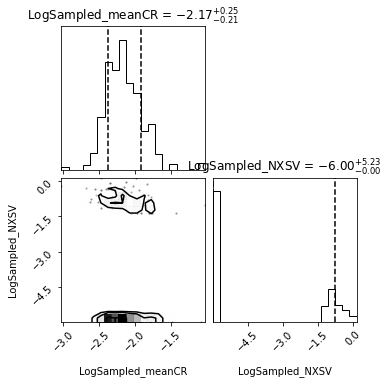
\includegraphics[width=0.47\linewidth]{Figures/Corner_all.png} }}%
    \qquad
    \subfloat{{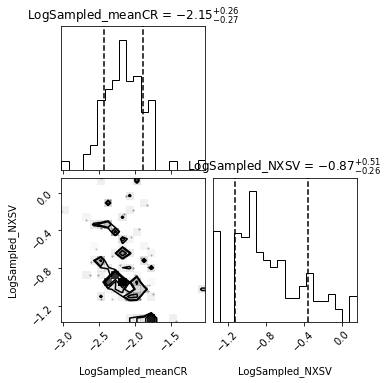
\includegraphics[width=0.47\linewidth]{Figures/Corner_nonzero.png} }}%
     \caption{Αριστερά: Τριγωνικό διάγραμμα \textlatin{(corner plot)} του παραμετρικού χώρου του αλγορίθμου μας- απεικονίζονται οι δύο παράμετροι $(CR_{mean}, \sigma_{rms}^2)$ σε λογαριθμική κλίμακα για όλες τις πηγές του πληθυσμού. Δεξιά: Τριγωνικό διάγραμμα \textlatin{(corner plot)} του παραμετρικού χώρου αποκλείοντας τις πηγές για τις οποίες ο αλγόριθμος απέδωσε την χαμηλότερη τιμη πλάτους μεταβλητότητας $\sigma_{rms, Bayes}^2 =10^{-6}$. Οι διακεκομμένες κατακόρυφες γραμμές ορίζουν το διάστημα γύρω από την μέση τιμή στο οποίο περικλείεται το $68\%$ (περίπου $1\sigma$) της κατανομής κάθε παραμέτρου.}  \label{fig:Corner}
\end{figure*}
  
%-------------------------------------------%
%-------------------------------------------%
%-------------------------------------------%

\section{Αποτελέσματα και σύγκριση με την βάση δεδομένων}

Αποτέλεσμα του αλγόριθμου αυτού με το πακέτο \textlatin{UltraNest} είναι για κάθε μία από τις 210 πηγές μας να έχουμε μία αλυσίδα \textlatin{Markov} me 3000 εως 5000 περίπου δείγματα τιμών $CR_{mean}$ και άλλη μία αλυσίδα \textlatin{Markov} me 3000 εως 5000 περίπου δείγματα τιμών $\sigma_{rms}^2$.

Ως τιμές δειγματοληψίας του αλγορίθμου για τις πηγές μας χρησιμοποιούμε τον αριθμητικό μέσο των τιμών της αλυσίδας $CR_{mean}$ με σφάλμα μέσης τιμής ως αβεβαιότητα και την επικρατούσα τιμή (\textlatin{mode}) των τιμών της αλυσίδας $\sigma_{rms}^2$ με το ελάχιστο διάστημα εμπιστοσύνης $68\%$ ($1\sigma$) του μαζικότερου όγκου της αλυσίδας. Την επικρατούσα τιμή και το διάστημα εμπιστοσύνης τα υπολογίζουμε αφού κάνουμε ένα ιστόγραμμα των καταμετρήσεων των τιμών τις αλυσίδας της διακύμανσης κατανεμημένο σε λογαριθμικό χώρο σε 500 ομάδες \textlatin{(bin)} ίσου λαγαριθμικού πλάτους. Ο μέσος της υψηλότερης \textlatin{bin} του ιστογράμματος θεωρείται η επικρατούσα τιμή \textlatin{(mode)}. Κανονικοποιούμε το ύψος των \textlatin{bin} ώστε να εκφρ'αζεται ώς ποσοστό της μοναδιαίας επιφάνειας του ιστογράμματος κι έπειτα ξεκινώντας από την υψηλότερη \textlatin{bin} συγκρίνουμε τις δύο εγγύτερες της (την εγγύτερη χαμηλότερων τιμών και την εγγύτερη υψηλότερων τιμών) και αθροίζουμε στο ύψος της το ύψος της επικρατέστερης των δύο, επαναλαμβάνουμε μέχρι το άθροισμα αυτό κανονικοποιημένων τιμών να φτάσει το $0.68$ (ελάχιστο διάστημα εμπιστοσύνης). Ως κάτω όριο του διαστήματος εμπιστοσύνης ορίζουμε το μέσο της κάτω χαμηλότερης \textlatin{bin} ενώ ως άνω όριο το μέσο της άνω χαμηλότερης \textlatin{bin} (με κέντρο την επικρατούσα τιμή). Για τις πηγές στις οποίες βρίσκουμε ότι η υψηλότερη \textlatin{bin} (στην οποία τον μέσο θα είχαμε την επικρατέστερη τιμή) έχει ήδη ύψος ίσο ή μεγαλύτερο του $0.68$ και είναι η \textlatin{bin} με τις χαμηλότερες τιμές $\sigma_{rms}^2$ της αλυσίδας δίνουμε ως επικρατούσα τιμή την ελάχιστη $10^{-6}$ kai ως κάτω όριο του διαστήματος εμπιστοσύνης επ'ισης $10^{-6}$. Στο σχήμα \ref{fig:Corner} βλέπουμε την κατανομή του παραμετρικού χώρου δύο διαστάσεων του αλγορίθμου μας. 

\begin{figure*}  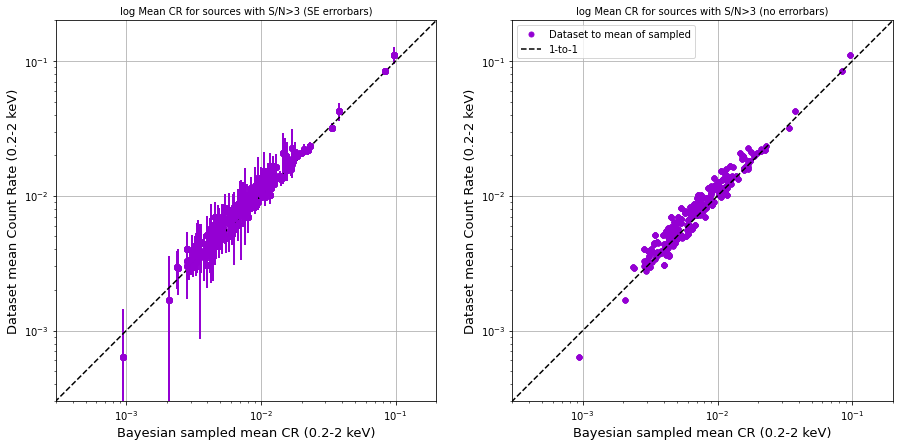
\includegraphics[width=1.12\linewidth]{Figures/Sampled Mean CR.png} \caption{Ο μέσος ρυθμός καταγραφής φωτονίων \textlatin{(mean CR)} όπως υπολογίσαμε από τα δεδομένα αρχείου με τον δειγματοληπτικό \textlatin{(mean CR)} από τον αλγόριθμο. Ως τιμή του δειγματοληπτικού αλγορίθμου έχουμε τον αριθμητικό μέσο της αλυσίδας \textlatin{Markov} κάθε πηγής με το σφάλμα μέσης τιμής ως αβεβαιότητα. Αριστερά έχουμε όλες τις πηγές μαζί με γραμμές σφαλμάτων, ενώ δεξιά έχουμε το ίδιο γράφημα χωρίς τις γραμμές σφαλμάτων.} \label{fig:SampledMeanCR}\end{figure*}

Κάνουμε το γράφημα μέσου ρυθμού καταγραφής φωτονίων της βάσης δεδομένων με τον μέσο ρυθμό καταγραφής φωτονίων που παρήξαμε από τον δειγματοληπτικό αλγόριθμο για να συγκρίνουμε αν τα αποτελέσματα είναι σε συμφωνία (Σχήμα \ref{fig:SampledMeanCR}). Ομοίως και για την παράμετρο $\sigma_{rms}^2$ (Σχήμα \ref{fig:SampledNXSV}).\\
Η τιμή ρυθμού καταγραφής φωτονίων υπολογισμένη από την βάση δεδομένων προκύπτει από την εξίσωση \ref{eq:CR} gia κάθε σημείο καμπύλης φωτός μίας πηγής. Η τιμή του μέσου ρυθμού καταγραφής φωτονίων της βάσης δεδομένων είναι ο αριθμητικός μέσος της ποσότητας \textlatin{CR} για όλα τα σημεία της καμπύλης φωτός μιας πηγής και το αντίστοιχο σφάλμα μέσης τιμής η απεικονιζόμενη αβεβαιότητα.\\
Η τιμή της εγγενούς διακύμανσης $\sigma_{rms}^2$ υπολογισμένη από την βάση δεδομένων (από τις καμπύλες φωτός) προκύπτει από την εξίσωση \ref{eq:NXSV} ενώ η αβεβαιότητα (γραμμές σφάλματος) σε αυτήν προκύπτει από την εξίσωση \ref{eq:NXSVerr} για κάθε πηγή και είναι η \textlatin{NXSV} όπως συζητήθηκε στην παράγραφο 5.2.4. Οι γραμμές σφάλματος για την \textlatin{NXSV} από τον δειγματοληπτικό αλγόριθμο σηματοδοτούν το ελάχιστο διάστημα εμπιστοσύνης ($68\% \; (1 \sigma)$ του μαζικότερου όγκου της αλυσίδας δειγματοληψίας για την \textlatin{NXSV}. Στο σχήμα \ref{fig:SampledNXSV} τα γραφήματα στο πάνω δεξιά \textlatin{panel} και κάτω δεξιά \textlatin{panel} περιέχουν όλες τις πηγές (πάνω με γραμμές σφαλμάτων και κάτω χωρίς γραμμές σφαλμάτων) όμως οι πηγές που έχουν \textlatin{NXSV} (κλασσικά υπολογισμένη ή από αλγόριθμο) με τιμή μικρότερη του $0.005$ εμφανίζονται στα επίπεδα $x=0.0001$ και $y=0.005$, για λόγους εξοικονόμισης χώρου.

\begin{figure*}  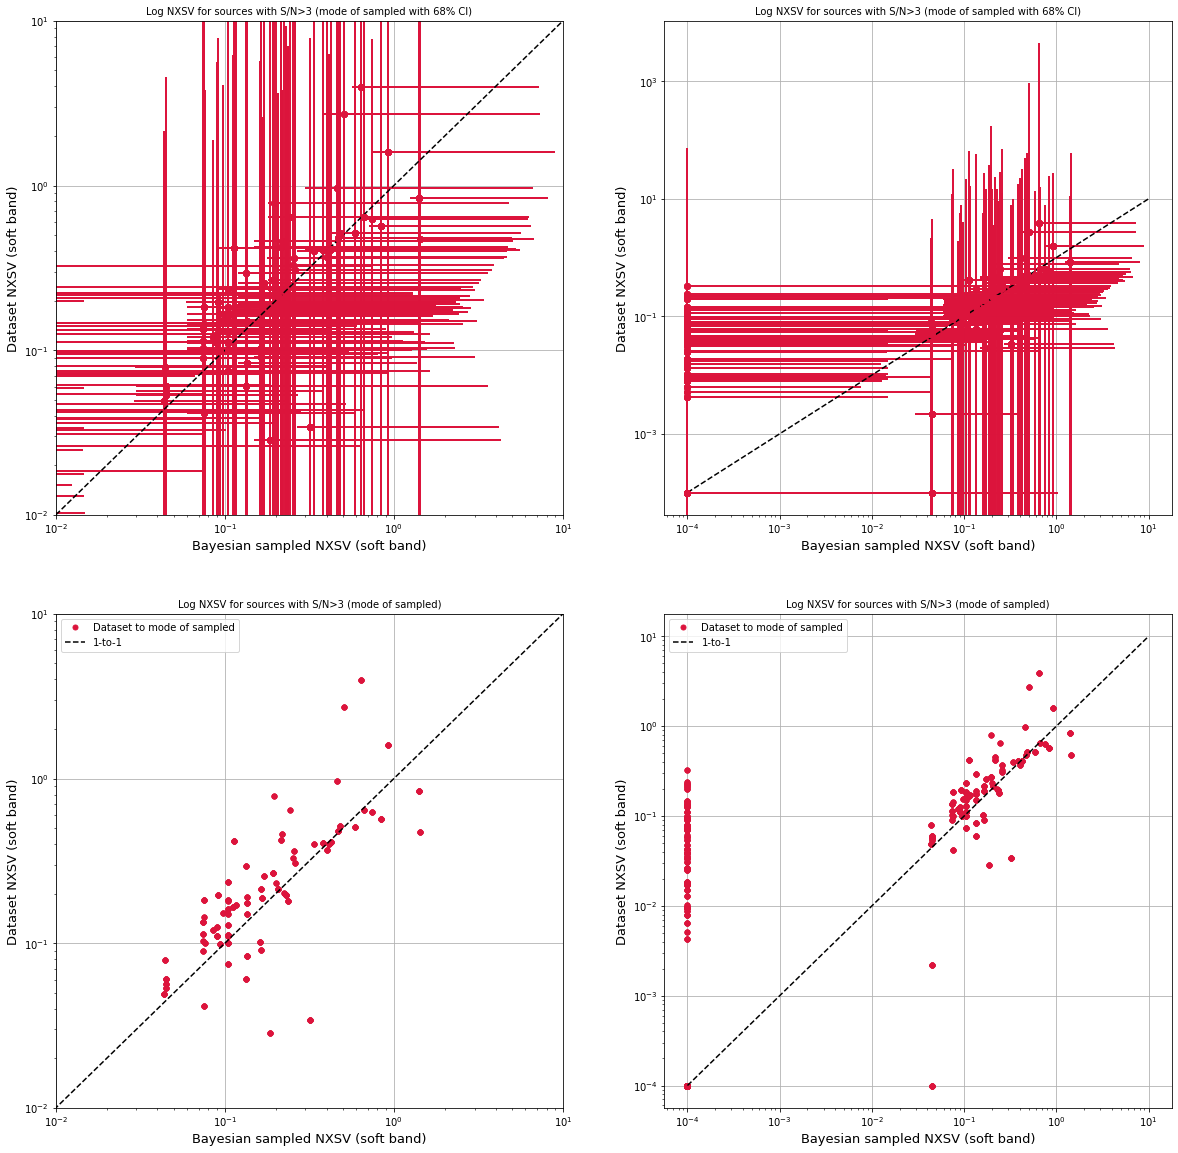
\includegraphics[width=1.12\linewidth]{Figures/Sampled NXSV trunc.png} \caption{H αναλυτική \textlatin{NXSV} όπως υπολογίσαμε από τα δεδομένα αρχείου (σε κάθε κατακόρυφο άξονα) με την \textlatin{NXSV} του δειγματοληπτικού αλγορίθμου συμπερασματολογίας \textlatin{Bayes} (σε κάθε οριζόντιο άξονα). Με διακεκομμένες γραμμές είναι η ένα προς ένα σχέση $y=x$. Ta κάτω πάνελ έχουν ακριβώς τις ίδιες πηγές και εύρος αξόνων με τα ακριβώς από πάνω, δεν έχουν όμως γραμμές σφαλμάτων. Στα πάνω πάνελ, αριστερά έχουμε τον κύριο όγκο των πηγών σε λογαριθμική κλίμακα με εύρος από $10^{-2}$ έως $10$, ενώ δεξιά έχουμε όλες τις πηγές απεικονίζοντας την \textlatin{NXSV} όπου αυτή είναι μικρότερη του $0.005$ στα επίπεδα $y=0.005$ (για την κλασσικά υπολογισμένη) kai $x=0.005$ (για την δειγματοληπτική του αλγορίθμου).} \label{fig:SampledNXSV} \end{figure*}

Παρατηρούμε ότι οι δειγματοληπτικές τιμές με τις κλασσικά υπολογισμένες τιμές συμφωνούν μέσα στα πλαίσια των γραμμών σφαλμάτων. Υπάρχουν πηγές για τις οποίες η δειγματοληπτική μέθοδος προβλέπει μικρότερο πλάτος \textlatin{NXSV} (σημεία στο γράφημα \ref{fig:SampledNXSV} που βρίσκονται πάνω από την γραμή σχέσης 1-1), όμως οι γραμμές σφάλματος περικλείουν την σχέση ταύτησης ένα-προς-ένα.
%({\color{red} νομιζω οτι πρεπει να πεις οτι υπαρχει συμφωνια μεσα στα σφαλματα. Υπαρχουν τιμες που βρισκονται πανω στιν 1-1 σχεση, αλλα και τιμες για τις οποιες η Μπαυζιανη μεθοδος βρισκει πολυ μικροτερο NXSV. Παρόλα'υτα για αυτες τις πηγες το σφαλμα ειναι συμφωνω με την 1-1 σχεση. Ισως αξιζει να βαλεισ τα αρνητικα NXSV στο 1ε-6 και να διξεις οτι υπαρχουν πηγες για τις οποιες η Μπευζιανη προβλεπη μεγαλα NXSV αλλα η κλασσικη μεθοδος οχι}). 

Προχωρούμε στο γράφημα εγγενούς διακύμανσης \textlatin{NXSV} με την λαμπρότητα των πηγών, συγκρίνουμε το γράφημα κλασσικά υπολογισμένης \textlatin{NXSV} με την λαμπρότητα (Σχήμα \ref{fig:ClassicResult}) με το γράφημα της δειγματοληπτικής \textlatin{NXSV} με την λαμπρότητα (Σχήμα \ref{fig:SampledResultB}). Από τις 210 πηγές με παρατηρήσεις απότον ανιχνευτή ΡΝ σε τρείς εποχές και με λόγο σήματος προς θόρυβο $>3$ οι 175 έχουν πληροφορία για ερυθρομετατόπιση (οπότε μόνο για αυτές έχουμε λαμπρότητα).\\ 
Στα γραφήματα αυτά ομαδοποιούμε τις πηγές σε ομάδες των 20 ξεκινώντας από τις χαμηλότερες λαμπρότητες (η τελευταία ομάδα- που αντιστοιχεί σε υψηλότερες λαμπρότητες έχει πάνω από 20 πηγές) και παίρνουμε τον αριθμητικό μέσο της \textlatin{NXSV} για τις συλλογές αυτές των πηγών. Οι γραμμές σφάλματος των σημείων \textlatin{ensemble NXSV} (από συλλογές 20 τουλάχιστον πηγών) προκύπτουν από σφάλμα μέσης τιμής. Αντίστοιχα για κάθε συλλογή υπολογίζεται ο αριθμητικός μέσος της λαμπρότητας. Οι γραμμες σφάλματος για την φωτεινότητα οριοθετούν το εύρος μέγιστης και ελάχιστης λαμπρότητας της συλλογής των πηγών.\\
Και στα δύο γραφήματα φαίνεται η αντισυσχέτιση της \textlatin{NXSV} με την λαμπρότητα, στο σχήμα \ref{fig:SampledResultB} φαίνεται πως για το αποτέλεσμα του αλγορίθμου έχουμε μια αμυδρή κλίση, ενώ στο σχήμα \ref{fig:ClassicResult} (το κλασσικό αποτέλεσμα) η αντισυσχέτιση είναι πιο έκδηλη.
%({\color{red} εξηγησε μεσες τιμες κλπ στα σχηματα}).

\begin{figure*} 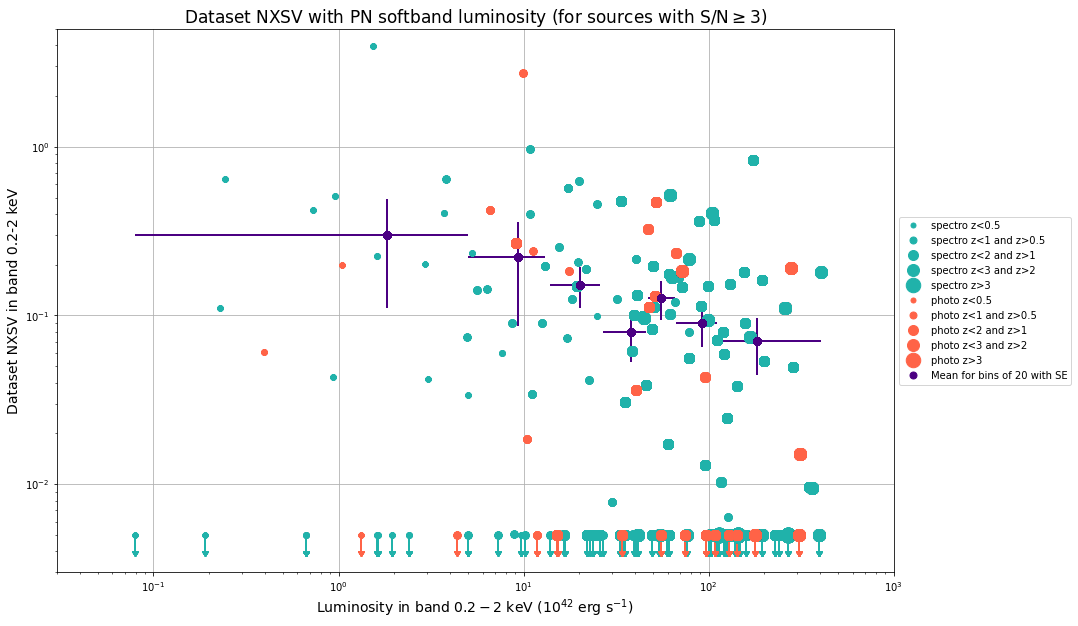
\includegraphics[width=1.12\linewidth]{Figures/Classic NXSV vs Lumi w BINS.png}\caption{H αναλυτική \textlatin{NXSV} όπως υπολογίσαμε από τα δεδομένα αρχείου με λαμπρότητα και \textlatin{binning} κατά λαμπρότητα σε \textlatin{bin} των 20 πηγών με διαφοροποίηση για \textlatin{redshift.}} \label{fig:ClassicResult}  \end{figure*}
 
\begin{figure*} 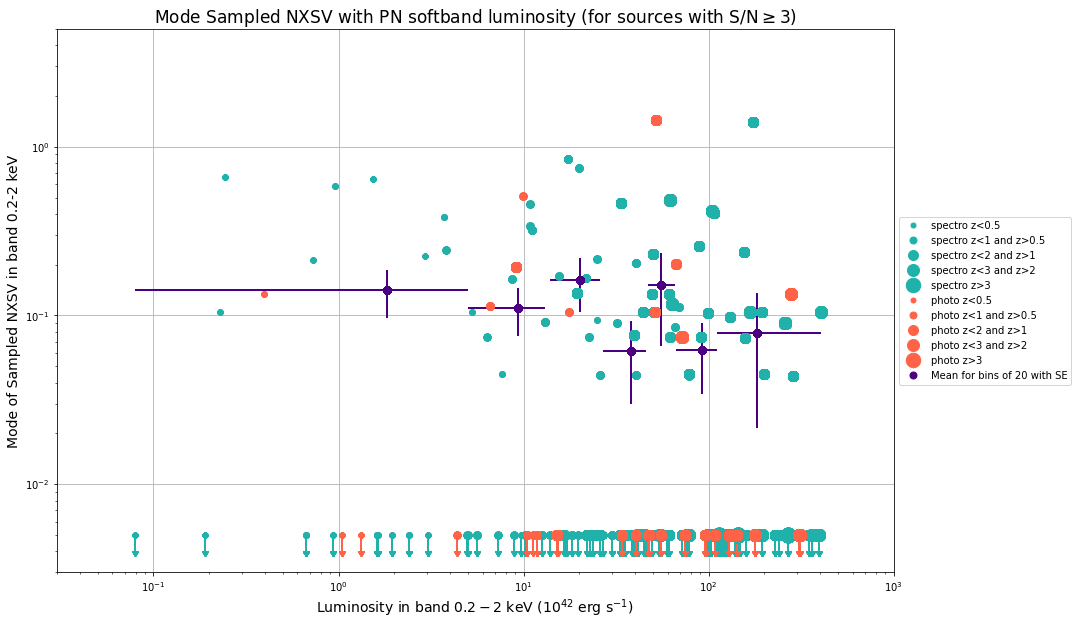
\includegraphics[width=1.12\linewidth]{Figures/Mode Sampled NXSV vs Lumi w BINS B.png} \caption{ Η \textlatin{NXSV} από τον αλγόριθμο \textlatin{Bayes} με λαμπρότητα και \textlatin{binning} κατά λαμπρότητα σε \textlatin{bin} των 20 πηγών με διαφοροποίηση για \textlatin{redshift.}} \label{fig:SampledResultB}  \end{figure*}
 
 
Προβαίνουμε σε στατιστικούς ελέγχους και απλή γραμμική προσαρμογή για να εξετάσουμε την σχέση δειγματοληπτικής \textlatin{NXSV} $\sigma_{rms, Bayes}^2$ με τον λογάριθμο της λαμπρότητας σε μαλακές ακτίνες Χ $\log L_X$. Ως αρχική υπόθεση ($P_{null}$) θεωρούμε ότι δεν υπάρχει συσχέτιση μεταξύ της \textlatin{NXSV} $\sigma_{rms, Bayes}^2$ και του $\log L_X$. Για το στατιστικό τεστ \textlatin{Kendall's} $\tau$ ο συντελεστής συσχέτισης $\sigma_{rms, Bayes}^2$ και $\log L_X$ για τις πηγές με φασματοσκοπικό $z$ είναι $\tau_{spectro} = -0.036$ ενώ για τις πηγές με φωτομετρικό $z$ είναι $\tau_{photo} = -0.053$ τα οποία αντιστοιχούν σε $P_{null, spectro} = 0.539$ kai $P_{null, photo} = 0.682$. Τα αρνητικά πρόσημα στους συντελεστές υποδηλώνουν φθίνουσα μονότονη σχέση, ενώ θεωρούμε ότι υπάρχει (αντι)συσχέτιση αν έχουμε τιμή σημαντικότητας $P_{null}<5\%$, το οποίο δεν ισχύει ούτε για τις πηγές με φασματοσκοπικό ούτε για τις πηγές με φωτομετρικό $z$. Το στατιστικό τεστ \textlatin{Spearman's rank} δίνει συντελεστή συσχέτισης $\rho_{spectro} = -0.048$ me $P_{null, spectro} = 0.573> 0.05$ για τις πηγές με φασματοσκοπικό \textlatin{redshift} kai $\rho_{photo} = -0.074$ me $P_{null, photo} = 0.686>0.05$ για τις πηγές με φωτομετρικό \textlatin{redshift}- δηλαδή δεν έχουμε συσχέτιση της $\sigma_{rms, Bayes}^2$ των πηγών με την λογαριθμική λαμπρότητα $\log L_X$. \\
Για το σύνολο των πηγών (ανεξαρτήτως διαχωρισμού \textlatin{redshift}), το τεστ \textlatin{Kendall's} $\tau$ δίνει συντελεστή συσχέτισης $\tau_{tot} = -0.032$ me $P_{null, tot}= 0.537 >0.05$ ενώ το τεστ \textlatin{Spearman's rank} δίνει συντελεστή συσχέτισης $\rho_{tot} =-0.047$ me $P_{null, tot} = 0.541>0.05$, οπότε και στο σύνολο των πηγών επιβεβαιώνεται η μη-συσχέτιση δειγματοληπτικής \textlatin{NXSV} και λογαριθμικής λαμπρότητας.\\
Για την \textlatin{ensemble NXSV} ο έλεγχος \textlatin{Kendall's} $\tau$ δίνει συντελεστή συσχέτισης $\tau = -0.238$ και ο έλεγχος \textlatin{Spearman's rank} δίνει συντελεστή συσχέτισης $\rho= -0.393$ me τιμές σημαντικότητας $P_{null, \tau} =0.562>0.05$ kai $P_{null, \rho} =0.383>0.05$ αντίστοιχα. Έχουμε δηλαδή μη-συσχέτιση της \textlatin{ensemble NXSV} με την λογαριθμική λαμπρότητα σε επίπεδο σημαντικότητας $95\%$. Η \textlatin{ensemble NXSV} μας επιτρέπει να ελαττώσουμε την διασπορά του δείγματος ώστε να φανεί τυχούσα υποβόσκουσα εξάρτηση. \\ 
Προσαρμόζουμε γραμμική σχέση μέσω γραμμικής παλινδρόμησης (\textlatin{linear regression}) sta δεδομένα και βρίσκουμε κλίση $-0.03$ (δηλαδή $\sigma_{rms, ensemble}^2 = \overline{\sigma_{rms}^2} \propto L_X^{-0.03}$) με σφάλμα μέσης τιμής $StErr = 0.02 $ για την \textlatin{ensemble NXSV}, φυσικά, η κλίση $-0.03$ με σφάλμα μέσης τιμής $0.02$ δεν είναι ικανή να υποστηρίξει συσχέτιση. 

Σε αντίθεση με το κλασσικό αποτέλεσμα, στην περίπτωση της δειγματοληπτικής \textlatin{ensemble NXSV} δεν υποστηρίζεται καμία συσχέτιση με την λαμπρότητα, έτσι συμπεραίνουμε ότι για τον αλγόριθμό που προσαρμόσαμε στα δεδομένα του δείγματός μας, οι \textlatin{AGN} διαφορετικής λαμπρότητας είναι εξίσου μεταβλητοί.\\
Ακόμα κι εδώ, όμως, η αβεβαιότητα των υπολογισμών- τόσο για την εκτίμηση της εγγενούς διακύμανσης κάθε μίας πηγής του δείγματός μας, όσο και τα σφάλαματα μέσης τιμής που αντιστοιχούν στην \textlatin{ensemble NXSV}- είναι τόσο μεγάλη που μας εμποδίζει να έχουμε ένα καταληκτικό συμπέρασμα. 